% Template for SLT-2006 paper; to be used with:
%          spconf.sty  - ICASSP/ICIP LaTeX style file, and
%          IEEEbib.bst - IEEE bibliography style file.
% --------------------------------------------------------------------------
\documentclass{article}
\usepackage{spconf,amsmath,epsfig}
\usepackage{amsmath,amssymb,amsthm,amsfonts,graphicx,hyperref,subfigure,rotating}
\renewcommand{\thefigure}{\arabic{figure}}

\usepackage{url}
%% Define a new 'leo' style for the package that will use a smaller font.
\makeatletter
\def\url@leostyle{%
  \@ifundefined{selectfont}{\def\UrlFont{\sf}}{\def\UrlFont{\small\ttfamily}}}
\makeatother
%% Now actually use the newly defined style.
\urlstyle{leo}

% Example definitions.
% --------------------
\def\x{{\mathbf x}}
\def\L{{\cal L}}

% Title.
% ------
\title{Image Matching using Scale Invariant Feature Transform (SIFT)}
% 
% Single address.
% ---------------
\name{Naotoshi Seo and David A. Schug}
\address{University of Maryland\\ENEE631 Digital Image and Video Processing\\Final Project\\Professor: Min Wu}
% 
% For example:
% ------------
% \address{School\\
%   Department\\
%   Address}
% 
% Two addresses (uncomment and modify for two-address case).
% ----------------------------------------------------------
% \twoauthors
% {A. Author-one, B. Author-two\sthanks{Thanks to XYZ agency for funding.}}
%	{School A-B\\
%   Department A-B\\
%   Address A-B}
% {C. Author-three, D. Author-four\sthanks{The fourth author performed the work
%     while at ...}}
%	{School C-D\\
%   Department C-D\\
%   Address C-D}
% 
\begin{document}
% \ninept
% 
\DeclareGraphicsExtensions{.pdf,.eps,.gif,.jpg,.eps, .png}
\maketitle
% 
\begin{abstract}
This paper explores the effectiveness of the Scale Invariant Feature Transform (SIFT) for image matching. 
There is a popularly used interest point detection method often applied to image matching, the Harris corner detector. 
The Harris corner detector is non-invariant to scale change. 
The experiments of image matching based on both the SIFT and the Harris corner detector are performed to show 
the effectiveness of the scale invariant property of the SIFT method. 
Furthermore, the image matching method based on SIFT is applied to point tracking, 
and comparison with Kanade-Lucas-Tomasi (KLT) feature point tracker is also studied. 

\end{abstract}
% 
\begin{keywords}
Image matching, interest point detection, point tracking, object tracking, panoramic image stitching

\end{keywords}
% 
\section{Introduction}
\label{sec:intro}

Image matching is a fundamental aspect of many problems in computer vision, including object or scene recognition, solving for 3D structure form multiple images, stereo correspondence, and motion tracking. 
Scale-invariant feature transform (or SIFT) proposed by David Lowe in 2004 \cite{dLowe04} is an algorithm for extracting interest point features from images that can be used to perform reliable matching between different views of an object or scene. 
The features are invariant to image scale, rotation, and partially invariant (i.e. robust) to change in 3D viewpoint, addition of noise, and change in illumination. 
They are well localized in both the spatial and frequency domains, reducing the probability of disruption by occlusion, clutter, or noise. Large numbers of features can be extracted from typical images with efficient algorithms. 
In addition, the features are highly distinctive, which allows a single feature to be correctly matched with high probability against a large database of features, providing a basis for object and scene recognition.

\section{Previous Works}\label{S:survey}

Several previous techniques related to SIFT were also examined. 

\subsection{Harris Corner Detector}\label{SS:Harris}


Corner detection or the more general terminology interest point detection is an approach used with computer vision systems to extract certain kinds of features and infer the contents of an image. 
There are several applications of interest point detection such as motion detection, tracking, image stitching, 3D modeling, and object recognition. 

An interest point is a point in an image which has a well-defined position and can be robustly detected. 
A corner is a feature often used as an interest point because of its locality, and orientation invariance. 
% A corner can be defined as the intersection of two edges. A corner can also be defined as a point for which there are two dominant and different edge directions in a local neighbourhood of the point. An interest point is a point in an image which has a well-defined position and can be robustly detected. This means that an interest point can be a corner but it can also be, for example, an isolated point of local intensity maximum or minimum, line endings, or a point on a curve where the curvature is locally maximal. 

Since the application of the Moravec interest operator in 1979 \cite{hMoravec79}, a lot of research has been done in corner and interest point detection. 
Harris corner detector \cite{cHarris88} proposed by Harris and Stephens in 1988 is a popularly used interest point detector. 



\subsubsection{How It Works}

Let the image given by $ I $. The Hessian matrix is given by 
\begin{equation}
  \mathbf{C} = \begin{bmatrix}
    \sum I_{x}^2 & \sum I_{xy}\\
    \sum I_{xy} & \sum I_{y}^2
  \end{bmatrix}.
\end{equation}
The summations are taken over a small region, and the derivatives are estimated by taking differences of neighboring points. 

The strength of the corner is determined by 'how much' second derivative there is. 
This is done by considering the eigenvalue ($ \lambda_1 $ and $ \lambda_2 $) of $ \mathbf{C} $. 
Based on the magnitudes of the eigenvalues, the following inferences can be made: \\
\indent 1. If $\lambda_1$ and $\lambda_2$ are both large, a corner is found. \\
\indent 2. If $\lambda_1 \gg \lambda_2 $ or $ \lambda_2 \gg \lambda_1 $, an edge is found. \\
\indent 3. If $\lambda_1$ and $\lambda_2$ are both small, there are no features of interest at this pixel $(x,y)$.

Thus, the strength of corner response can be computed by
\begin{equation}
  R = \lambda_1 \lambda_2 - \kappa \, (\lambda_1 + \lambda_2)^2.
\end{equation}
where $\kappa$ is a tunable parameter which determines how 'edge-phobic' the algorithm is.

Harris and Stephens note that exact computation of the eigen values is computationally expensive and instead suggest the
following function, 
\begin{equation}
  R = Det(\mathbf{C}) - \kappa \, Tr^2(\mathbf{C})
\end{equation}
because $ Det(\mathbf{C}) = \lambda_1 \lambda_2 $ and $ Tr(\mathbf{C}) = \lambda_1 + \lambda_2 .$

The value of $\kappa$ has to be determined empirically, and in the literature values in the range 0.04 - 0.15 have been reported as feasible.

\subsubsection{Discussion}

As mentioned, a corner is well localized, and invariant to rotation. 
Furthermore, Harris corner detector is partially invariant to affine intensity change (translation or scaling in the intensity domain) because only derivatives of intensities are used. 
However, Harris corner detector is non-invariant to image scaling. 
This defect is resolved by SIFT. 

\begin{figure}[ht]
  \begin{center}
    \scalebox{1.0}{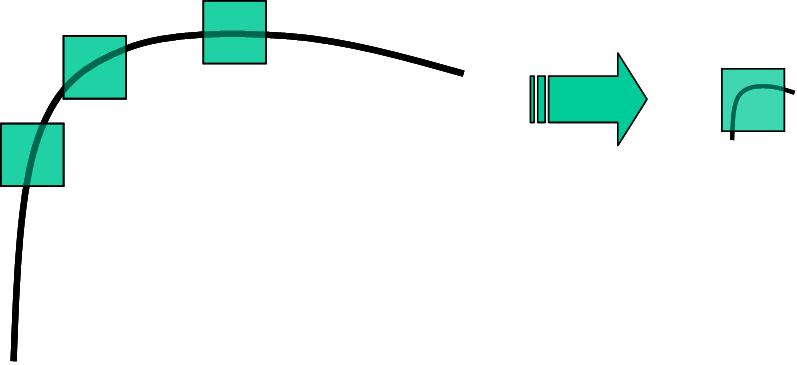
\includegraphics[width=7cm]{../HarrisScaleVariant.png}}
  \end{center}
  \caption{An example showing scale non-invariant property. Left: Edges. Right: A corner. Edges are recognized as a corner by scaling down}
  \label{fig:HarrisScaleVariant}
\end{figure}

\subsubsection{Application to Image Matching}\label{SSS:HarrisImageMatch}

After detecting interest points in two images, we are possibly able to find corresponding points in the two images. 
This process is called as image matching and it can furthermore applied for image stitching, point tracking, automatic determination of epipolar geometry. 

There are several image matching methods based on Harris Corner detector, affine invariant \cite{tTuytelaars00}, rotation invariant  \cite{jMatas03}, and deformation invariant \cite{hLing05} methods. 
But, we simply compute Sum of Squared Difference (SSD) within a small search window around the detected corner pairs in the two images. 
Then we recognize two points as a corresponding pair if their SSD is the smallest among other corner points. 
This method is translation invariant, but non-invariant to image rotation, and scale. 

\subsection{Kanade-Lucas-Tomasi (KLT) Feature Tracker}

The {\bf KLT} tracker is used to derive interesting features and follow them through an image sequence. The collection of feature points can then be applied to typical computer vision problems as object recognition, tracking or structure from motion.
\cite{bLucas81} \cite{cTomasi91} \cite{jShi94} \cite{sBirchfield97}.

\subsubsection{Image Motion Models}
For a simplified feature based tracker two motion models are required: a local model to monitor tracking quality by measuring image dissimilarities between feature windows (registration problem) and an affine map model to compute displacement vectors (tracking problem).  The goal is to find the displacement ${\bf d}$ of a window center point $x = (u,v)$ on a feature image patch.  Because individual pixels can change with noise and be confused with neighbors or move out of view from frame to frame, it is necessary for the tracker to examine features through a window of pixels. Patterns move in the image stream according to function $I(u,v,t)$ and satisfies 
\[
I(u,v,t+\tau) = I(u-\xi(u, v, t, \tau),v-\eta(u, v, t, \tau),t).
\]
The next image $J({\bf x}) = I({\bf x},t+\tau)$ at time $t + \tau$, which can be obtained by moving every point in the image at time $t$ by a certain amount.  The amount of motion ${\delta} = (\xi, \eta)$ is the displacement of the image point $x = (u,v)$ between times $t$ and $t + \tau$.  The vector ${\delta}$ is a function of the image position ${\bf x}$, so there exist different displacements within the same window.  Actual tracking is modeled with an affine motion field
\[
\delta = D{\bf x} + {\bf d},
\] 
where
\[
D =
\begin{bmatrix}
  d_{uu} & d_{uv} \\
  d_{vu} & d_{vv} 
\end{bmatrix}
\]
is a deformation matrix and ${\bf d}$ is the displacement of the window center, as stated previously.   Image coordinates ${\bf x} = (u,v)$ are measured with respect to the window's center.  Thus, ${\bf x}$ in the first image $I$ moves to point $A{\bf x}+{\bf d}$ in second image $J$, where $A = {\bf 1}+D$ and ${\bf 1}$ is the $2\times 2$ identity matrix.     Therefore, we have that
\[
J(A{\bf x + d}) = I({\bf x }) + n({\bf x})
\]
where {\em n} is noise as a function of its position in the image frame.  Given two images $I$ and $J$, and a feature window in $I$, we define tracking to be the determination of the 6 parameters found in $D$ and ${\bf d}$. Camera motion, image texture, and window size influence the estimates.  When the window is small, $D$ is harder to estimate since the variations of motion are small and less reliable.  Small windows will prevent depth discontinuities so we often use a pure translation model with deformation matrix $D$ set to zero and $\delta = {\bf d}$.  This model works for tracking and is reliable over small interframe camera motion while the affine model can be added to monitor tracking quality. 

To solve the registration problem we monitor residuals.  The image $J$ can be thought of as an intensity function depending upon ${\bf x} = (u,v)$.  Then, when image displacements are small, the image intensity function $J$ can be approximated by a Taylor series expansion truncated to the linear term
\begin{equation}
  J({\bf x + d}) = J({\bf x}) + {\bf g}^T,\label{eq:taylor}
\end{equation}
where {\bf g} is the image gradient given by
\[
{\bf g} =
\begin{bmatrix}
  \partial_u I\\
  \partial_v I
\end{bmatrix}.
\]
The dissimilarity (registration) problem is that of finding the ${\bf d}$ that will minimize the residual error $\epsilon$ given a window $\mathcal{W}$ by calculating
\begin{equation}
  \epsilon = \iint_{\mathcal{W}}[J(A{\bf x + d})- I({\bf x})]^{2} w({\bf x})d{\bf x},
  \label{eq:epserror}
\end{equation}
where {\em w} is a weighting function that is usually set to 1, but could be a Gaussian that best represents the central area of the feature window ${\mathcal{W}}$.

% alogorithm

\subsubsection{Algorithm}
To compute image motion we must set up and solve the linear system to determine the motion parameters found in ${\bf A}$ above and ${\bf d}$ that will minimize the {\em dissimilarity} in (\ref{eq:epserror}).  When looking for a pure translation we let A be the identity matrix.  To minimize the residual in (\ref{eq:epserror}) we differentiate it with respect to the unknown entries of the deformation matrix D and the displacement vector ${\bf d}$ and set the result to zero.  Linearizing the resulting system with a truncated Taylor expansion, as in (\ref{eq:taylor}), we get the 6x6 linear system
\begin{equation*}
  T{\bf z = a}, 
\end{equation*}
where ${\bf z}^T = [d_{uu}\quad d_{vu}\quad d_{uv}\quad d_{vv}\quad d_u\quad d_v]$ contains the entries of deformation matrix D and displacement vector ${\bf d}$, and the error vector
\begin{equation}
  {\bf a} = \iint_{\mathcal{W}}[I({\bf x})- J({\bf x})]\begin{bmatrix}
    u {\bf g}\\
    v {\bf g}\\
    {\bf g}
  \end{bmatrix}
  w({\bf x})d{\bf x}
  \label{eq:erra}
\end{equation}
is dependent on the image difference and T, which can be computed from one image and expressed as
\begin{equation}
  T = \iint_{\mathcal{W}}\begin{bmatrix}
    U & V\\
    V^T & Z\\
  \end{bmatrix}
  w({\bf x})d{\bf x}
  \label{eq:paramT}
\end{equation}
where
\[
Z = {\bf g g}^T = 
\begin{bmatrix}
  \partial_{u}^2 I & \partial_{uv} I \\
  \partial_{uv} I & \partial_{v}^2 I
\end{bmatrix},
\]
\[
U =
\begin{bmatrix}
  u^2 Z &uv Z \\
  uv Z  &v^2 Z \\
\end{bmatrix}, \text{ and}
\]
\[
V^T =
\begin{bmatrix}
  u Z &v Z 
\end{bmatrix}.
\]
This full affine motion system is useful when  monitoring features for dissimilarities.  For tracking to determine ${\bf d}$, it is better to solve the smaller system
\begin{equation}
  Z{\bf d} = {\bf e}
\end{equation}
where {\bf e} collects the last 2 elements of vector {\bf a} in equation (\ref{eq:erra}).  During interframe tracking image motion is small and D is hard to estimate and nearly singular. D interacts with displacement ${\bf d}$ through matrix V of equation (\ref{eq:paramT}) and any error in deformation matrix D will cause errors in ${\bf d}$.  Next we must consider what features are worth tracking in an image.  This is done using the symmetric 2x2 matrix $Z$, which  must be above the noise level and well conditioned. To satisfy noise requirements both eigenvalues of $Z$ must be large, and to be well conditioned means that the eigenvalues cannot differ by several orders of magnitude. Two small eigenvalues signal an approximately constant intensity profile within a window. A large and a small eigenvalue indicates a unidirectional texture, and two large eigenvalues represent corners, salt and pepper textures, or some other reliable feature.  Intensity variations are bounded by a maximum allowable pixel value, so the eigenvalues are bounded.  Finally if the two eigenvalues of $Z$ are $\lambda_1$ and $\lambda_2$ we accept the window if
\begin{equation}
  min(\lambda_1,\lambda_2) > \lambda
\end{equation}
where $\lambda$ is a predefined threshold.  By computing the dissimilarity with the full affine map we can monitor residuals and occlude those features that have dissimilarities above a certain threshold.
\subsubsection{Occlusion handling}
A statistical based occlusion handling routine was implemented to filter outlier track points.  Given two images $I_n$ and $I_{n+1}$ and a feature list of $k$ corresponding tracked points present in both images, compute the interframe displacement $d_k$ of each feature. Next find the mean $\mu$ and standard deviation $\sigma^2$ and compute the $z$-score
\[
z_k = \frac{d_k - \mu}{\sigma}
\]
Any $d_k$ that exceeds 3.25 standard deviations, such that $z_k >3.25$, is then occluded.  These steps are implemented over the entire image sequence to filter outliers that could deteriorate tracking quality over the entire image sequence.

\subsubsection{Experiments and Results}

KLT Detector functions were applied, and experiments were performed for an image and its scale downed image (25\%).
The results are shown at Fig. \ref{Fi:hoteltracks}. 

\subsubsection{Discussion}
The KLT tracker is an important automation step in that it finds certain features to track and will follow them through the image sequence as long as image contrast, noise, and illumination is relatively constant and low.  If affine changes are large it is subject to drift, jump track if substantial clutter enters the scene, or occlude points entirely when there is a shadow or other illumination change.  For example, when tracking a bowtie if another object with a similar feature or corner comes into view it can choose that feature on the other object and begin tracking it instead. In many cases the matrix $Z$ defined above may be ill-conditioned and the eigenvalues may not be above the threshold requirement $min(\lambda_1,\lambda_2) > \lambda$ and occlude a point otherwise  observable by a human.  Also when another feature in the window satisfies the requirement to minimize $\epsilon$ in (\ref{eq:epserror}) the wrong feature displacement $\bf d$ is computed drift observer perceived drift takes at best. At worst the new counterfeit image point in the window satisfies the minimal requirement and the jump track case takes place.  SIFT was implemented to be more robust in the presence larger amounts of clutter, rotation, and illumination changes. 

\section{Scale Invariant Feature Transform}\label{S:SIFT}

The SIFT \cite{dLowe04} is a method for extracting interest point features from images, that is, 
it not only detects interest point locations but also extracts features around the points that can be used to perform reliable matching between different views of an object or scene. 
The SIFT features are invariant to not only to image orientation but also image scale, and provide robust matching across a substantial range of affine distortion, change in 3D viewpoint, addition of noise, and change in illumination. 

For image matching, SIFT features are first extracted from a set of reference images and stored in a database. A new image is matched by individually comparing each feature from the new image to this previous database and finding candidate matching features based on Euclidean distance of their feature vectors. 

\subsection{Algorithm Steps}

The major steps in the computation of SIFT are \cite{dLowe04}

\begin{enumerate}
\item \textbf{Scale-space construction} - construction of Gaussian and difference-of-Gaussian pyramids. 
\item \textbf{Keypoint localization} - keypoint candidates are chosen from the extrema in the scale space, and keypoints are selected based on measures of their stability. 
\item \textbf{Orientation assignment} - orientations are assigned to each keypoint based on histograms of gradient directions computed in a 16x16 window. 
\item \textbf{Keypoint descriptor} - representation in a 128-dimensional vector.
\end{enumerate}

\noindent\textbf{Keypoint matching} - the best candidate match is found by its nearest neighbor.

\subsection{Scale-Space Construction}\label{SS:DSSE}

\begin{figure*}[ht]
  \begin{center}
    \scalebox{1.0}{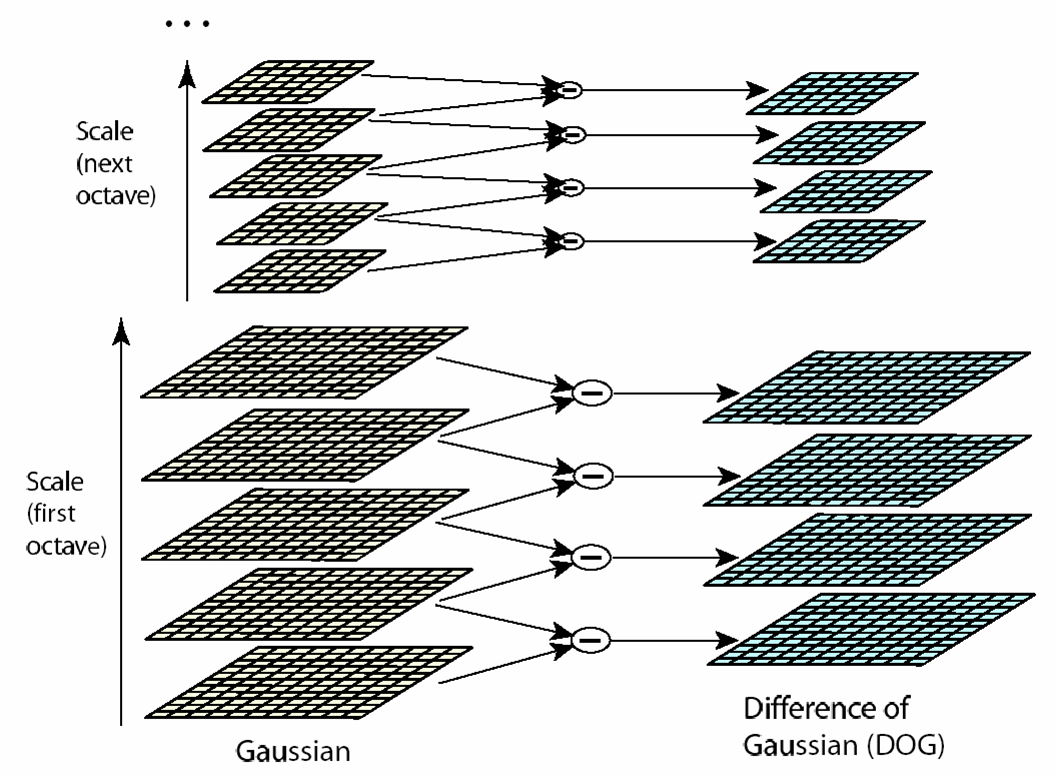
\includegraphics[width=12cm]{Pyramid.png}}
  \end{center}
  \caption{Gaussian and DoG Pyramids}
  \label{Fi:DOG}
\end{figure*}

Interesting image features or {\em key points} are detected using a cascade filtering approach that identifies image candidate locations that will be evaluated further later. 
The first step is to realize image location coordinates and scales that can be repeatably assigned under pose variation of the object of interest.  
Finding locations that are invariant to scale is performed by scale function that searches for stable features across different scales.  
The scale space convolution kernel of choice is the Gaussian function used to define the scale space function of an input image according to
\begin{equation}
  L(x,y,\sigma) = G(x,y,\sigma)\ast I (x,y)
\end{equation}
where $\ast$ is the convolution operation in $x$ and $y$ with Gaussian

\begin{equation}
  G(x,y,\sigma) = \frac{1}{2\pi \sigma}e^{-(x^2+y^2)/2\sigma^2}
\end{equation}
To detect stable keypoint locations in scale space, the difference-of-Gaussian (DoG) function convolved with the image $D(x,y,\sigma)$ is computed from the difference of two nearby scales separated by a constant multiplicative factor $k$ as in
\begin{align}
  D(x,y,\sigma) &= (G(x,y,k\sigma)-G(x,y,\sigma))\ast I(x,y)\\
  &= L(x,y,k\sigma)-L(x,y,\sigma).
\end{align}

The DOG function is a close approximation to the scale-normalized Laplacian of Gaussian $\sigma^2\nabla^2G$.  
It is known that the maxima and minima of $\sigma^2\nabla^2G$ produce the most stable image features compared to a range of other possible image functions, such as the gradient, Hessian, or Harris corner function. 

An approach to construction of $D(x,y,\sigma)$ is shown in Fig. \ref{Fi:DOG}. 
The input image is incrementally convolved with Gaussians using $ \sigma = \sqrt{2} $ to produce images shown stacked in the left column. 
That is, the bottom image is first convolved with Gaussian using $ \sigma = \sqrt{2} $, 
and then repeated with a further incremental smoothing of $\sigma = \sqrt{2}$ to give the 2nd bottom image, which now has an effective smoothing of $ \sigma = 2 $. 
The bottom DoG function is obtained by subtracting the 2nd bottom image from the bottom image, resulting in a ratio of $ 2 / \sqrt{2} = \sqrt{2} $ between the two Gaussians. 
We repeat these procedures until we generate $s+3$ images in the stack of Gaussian images and thus $s+2$ images in the stack of DoG images on each pyramid level or octave where $s$ is the number of intervals which we used 2 in our experiment. 
Fig. \ref{Fi:EXT} shows one interval of local extrema computation which uses 3 levels of DoG function. 

\begin{figure}[ht]
  \begin{center}
    \scalebox{1.0}{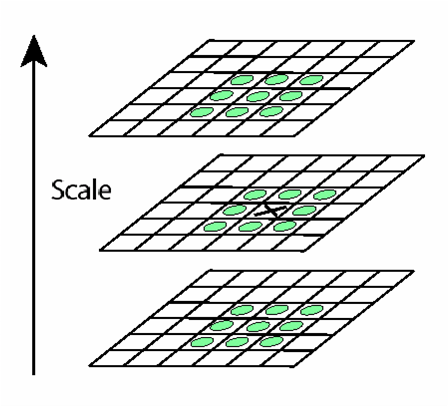
\includegraphics[width=5cm]{Extrema.png}}
  \end{center}
  \caption{One interval of local extrema detection}
  \label{Fi:EXT}
\end{figure}

To generate the next pyramid level, we downsample the bottom image of the current level by taking every second pixel in each row and column, which now has twice the initial value of $ \sigma $, that is, has an effective smoothing of $ \sigma = 2 \sqrt{2} $. 
Then, the same computations are repeated until we obtain the specified number of pyramid levels which we used 4 in our experiment. 

\subsection{Keypoint Localization}

\subsubsection{Local Extrema Detection}\label{SSS:LED}
Local maxima and minima of the DoG function are detected as keypoint candidates. 
To detect local maxima and minima of the DoG function, $D(x,y,\sigma)$, each sample point is compared to its eight nearest neighbors in the current image and nine neighbors in the scale above and below as in Fig. \ref{Fi:EXT}. 
Selection takes place only when a sample point is larger or smaller than all neighbors under comparison. 

To detect extrema reliably, the right frequency of sampling must be chosen in the image and scale domain. 
We can determine the best choices experimentally and the experiments were provided by \cite{dLowe04}. 
Lowe shows 3 intervals on each pyramid level is the best, but 2 is also reliably good. We chose 2 to reduce the computation time. 
Lowe also shows, as the total number of pyramid levels are increased, the total number of keypoints is increased, but the percent of correctness (repeatability) are decreased. 
He suggested to use 4 levels, and we also used 4. 
Lowe also suggests to prior blur with $ \sigma = 0.5 $ to prevent aliasing
and then upsample the image by a factor of 2 using linear interpolation. 
Lowe claims that the image doubling increase the number of stable keypoints by almost a factor of 4.

\subsubsection{Rejecting Low Contrast Keypoints}\label{SS:AKL}
Once a keypoint candidate has been realized, the next step is to perform a detailed fit to local image data for location, scale ,and ratio of principal curvatures. 
With this information points are rejected that have low contrast because they are sensitive to noise or are poorly localized along an edge.  

A simple approach of the implementation is to locate keypoints at the location and scale of the central sample point. 
There is another advanced approach which fit a three dimensional quadratic function to the local sample points to determine the location of the maximum. 
This approach provides improvements to matching and stability.  

This approach uses a Taylor expansion (up to the quadratic terms) of the scale-space function $D(x,y,\sigma)$ is shifted so the origin is located at the sample point

\begin{equation}
  D(\mathbf{x}) = D + \frac{\partial D^T}{\partial{ \mathbf{x}}}\mathbf{x} + \frac{1}{2}\mathbf{x}^T\frac{\partial^2 D}{\partial\mathbf{x}^2}\mathbf{x}
\end{equation}\label{eq:dxt}
where $D$ and its derivatives are evaluated at the sample point and $\mathbf{x} = (x,y,\sigma)^T$ is the offset from the particular point.  
The location of the extremum $\mathbf{\hat{x}}$ is determined by taking the derivative of $D$ with respect to $\mathbf{x}$ and setting it to zero such that
\begin{equation}
  \mathbf{\hat{x}} = \frac{\partial^2 D^{-1}}{\partial\mathbf{x}^2}\frac{\partial D}{\partial{ \mathbf{x}}}
\end{equation}\label{eq:dxth}
In practice the Hessian and derivative of $D$ are approximated by using differences of neighboring sample points, resulting the solution of a $3\times 3$ linear system.  When the offset, $\mathbf{\hat{x}}$ is larger than 0.5 in any dimension, then the implication is that the extremum lies closer to a different sample point.  In this case it is necessary to change sample points and interpolation is performed about the point instead.  The final offset $\mathbf{\hat{x}}$ is added to the location of its sample point to get the interpolated estimate for the location of the extremum.

By taking the function value at the extremum,  $D(\mathbf{\hat{x}})$, it is possible to reject unstable extrema with low contrast by substitution of equation (\ref{eq:dxth}) into (\ref{eq:dxt}) as in  
\begin{equation}
  D(\mathbf{\hat{x}}) = D + \frac{1}{2}\frac{\partial D^T}{\partial\mathbf{x}}\mathbf{\hat{x}}
\end{equation}
Lowe suggested to discard extrema with a value $|D(\mathbf{\hat{x}})| < 0.03$ by experiments. 

\subsubsection{Eliminating Edge Responses}\label{SSS:EER}
Using low contrast rejecting criteria alone is not sufficient because the DoG function will have a strong response at edges even when the location along the edge is poorly determined and therefore sensitive to small amounts of noise.  

As we've studied in Harris corner detector (Sec. \ref{SS:Harris}), it is possible to detect edges by a $2 \times 2 $ Hessian matrix. 

A poorly defined peak in the difference-of-Gaussian function will have a large principal curvature across the edge but a small curvature in the perpendicular direction. 
Principal curvatures are computed from the Hessian matrix

\begin{equation}
  \mathbf{H} = \begin{bmatrix}
    D_{xx} & D_{xy}\\
    D_{xy} & D_{yy}
  \end{bmatrix}
\end{equation}
where the derivatives are found by taking differences of neighboring points.  The eigenvalues of $\mathbf{H}$ are proportional to the principal curvatures of $D$.  It is not necessary to compute the eigenvalues explicitly as only the ratio is interesting.  Letting $\alpha$ be the eigenvalue with largest magnitude and $\beta$ the smaller, then the sum of eigenvalues is the trace of $\mathbf{H}$ 
\begin{equation}
  Tr(\mathbf{H})= D_{xx}+D_{yy}=\alpha + \beta
\end{equation}
and the product is the determinant
\begin{equation}
  Det(\mathbf{H})= D_{xx}D_{yy} - (D_{xy})^2=\alpha\beta
\end{equation}
When the determinant is negative, then the curvatures have different signs so the point is discarded as a candidate extremum.  Letting $r$ be the ratio between the largest magnitude eigenvalue and the smaller one such that $\alpha = r\beta$ then
\begin{align}
  \frac{Tr(\mathbf{H})^2}{Det(\mathbf{H})} &= \frac{(\alpha + \beta)^2}{\alpha \beta}\\
  &= \frac{(r\beta + \beta)^2}{r\beta^2}\\
  &= \frac{(r+1)^2}{r},
\end{align}
depending only on the ratio of the eigenvalues instead of their individual values.  When the two eigenvalues are equal the quantity $(r+1)^2/r$ is a minimum and will increase with $r$.  As a result to make sure the ratio of principal curvatures is below some threshold, $r$ it is necessary to check,
\begin{equation}
  \frac{Tr(\mathbf{H})^2}{Det(\mathbf{H})} < \frac{(r+1)^2}{r}. \label{eq:curveratio}
\end{equation}
Lowe suggested to choose $r=10$, which eliminates keypoints that have a ratio obtained by (Eq. \ref{eq:curveratio}) greater than 10. 



\subsection{Orientation Assignment}\label{SS:OA}
Consistent orientations based on local image properties are assigned to each keypoint. 
Representing the following keypoint descriptor relative to the orientation assignment is a motivating factor to help achieve invariance to image rotation.  

The scale of the keypoint is used to select the Gaussian smoothed image, $L$ with the closest scale, so that all computations are performed in a scale invariant manner.  
For each image sample, $L(x,y)$ at a particular scale the gradient magnitude, $ m(x,y) $, and orientation, $ \theta(x,y) $, is precomputed: 
\begin{equation}
  m(x,y) = \sqrt{L_x^2 + L_y^2 }
\end{equation}
\begin{equation}
  \theta(x,y) = \tan^{-1}(L_y/L_x)
\end{equation}
where $ L_x = L(x+1,y)-L(x-1,y) $ and $ L_y = L(x,y+1)-L(x,y-1) $ are pixel differences. 

An orientation histogram is formed from the gradient orientations of sample points within a region around the keypoint.  The orientation histogram has 36 bins covering  the 360 degree range of orientations.  
Also each sample added to the histogram is weighted by its gradient magnitude and by a Gaussian-weighted circular window with a $\sigma$ that is 1.5 times that of the scale of the keypoint. 

The peaks in the orientation histogram correspond to the dominant directions of local gradients. 
The highest peak in the histogram is detected, and then any other local peak that is within 80\% of the highest peak is used to also create a keypoint with that orientation.  
Therefore, for multiple peaks of similar magnitude, there will be multiple keypoints created at the same location and scale but different orientations. 
Finally a parabola is fit to the 3 histogram values closest to each peak to interpolate the peak position for improved accuracy.


\subsection{The Local Image Descriptor}\label{SS:LID}

\begin{figure*}[ht]
  \begin{center}
    \scalebox{1.0}{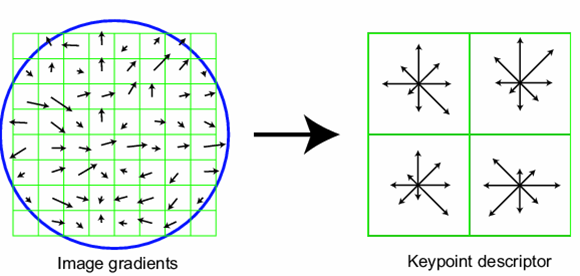
\includegraphics[width=10cm]{KeypointDescriptor.png}}
  \end{center}
  \caption{Keypoint descriptor process}
  \label{Fi:KDP}
\end{figure*}

After image location,scale, and orientation have been assigned to each keypoint, it is possible to impose a two dimensional coordinate system to describe the local image region and provide invariance with respect to these parameters.  
The next step is to compute a descriptor for the local image region that is distinct yet invariant to additional variations such as change in illumination and three dimensional pose.  

The traditional approach is to sample the local image intensities around the keypoint at the appropriate scale and matching with a normalized correlation measure.  
This has limitations as it is highly sensitive to changes in the image that cause misregistration of samples such as in affine or three dimensional pose variations and random noise interference.  
The better approach is to allow the gradient at a particular orientation and spatial frequency to shift locations over a small field rather than being precisely localized allowing for matching and recognition of three dimensional objects from a range of viewpoints.  
The claim is that matching gradients while allowing for shifts in their position results in better classification under three dimensional rotation.

\subsubsection{Descriptor Representation}\label{SSS:DR}
To begin representing a keypoint descriptor it is necessary to sample the image gradients and orientations around the keypoint location by applying the scale of the keypoint to determine the level of Gaussian blur for the image.  
Orientation invariance is achieved by rotating the coordinates of the descriptor and the gradient orientations relative to the keypoint orientations.  

Each sample point magnitude is assigned a weight by applying a Gaussian weighting function with $\sigma$ equal to one half the width of the descriptor window.  The purpose of the Gaussian window is to avoid sudden changes in the descriptor with small changes in the position of the window and deemphasize those gradients far from the center of the descriptor.  By generating orientation histograms over $4\times 4$ sample regions, it is possible to allow for large shifts in gradient positions.  
There are eight directions for each orientation histogram and the length of the arrow corresponds to the magnitude of a particular histogram entry.  A gradient sample can shift up to four positions and still participate in the histogram on the right thus allowing for larger positional shifts.

To avoid boundary affects where the descriptor changes from one histogram or orientation to another, trilinear interpolation is applied to distribute the value of each gradient sample into adjacent histogram bins.  
Each value in a bin is multiplied by a weight of $1-d$ for each dimension, $d$ being the distance of the sample from the central value of the bin based on the histogram bin spacing. 

For a descriptor it is necessary to form a vector of all orientation histogram entries.  
Lowe \cite{dLowe04} used a $4\times 4$ array of histograms with eight orientations in each bin, consequently each descriptor vector for a particular keypoint will be of length $4\times 4 \times 8 = 128$. 

To limit the effect of illumination changes the descriptor vector must first be normalized to unit length. 
When image contrast is represented by multiplying each pixel value some constant then he vector normalization will cancel changes because the gradient is multiplied by the same constant. Likewise changing contrast with addition of a constant to each pixel value will not affect gradient values because they a computed from pixel differences.  In either case the descriptor will be invariant to affine changes in illumination.

Finally it is necessary to manage the effects of nonlinear illumination changes that affect 3D surfaces by different orientations and magnitudes. Such illumination effects cause large change in relative magnitudes but not orientations.  Consequently large gradient magnitudes are thresholded by a factor of 0.2 and the entire feature vector is renormalized.  This factor determined experimentally. 

%To summarize the descriptor algorithm, ~\ref{Alg:DESC}
%\begin{figure}[ht]
%\centering
%\begin{list}{}{\setlength{\leftmargin}{2in}
%							 \setlength{\rightmargin}{1in}}
%	\item[Generate orientation histograms bins (default 8)]
%	\item[Create feature grid with $n\times n$ cells]
%	\item [For all of the keypoints]
%	\item[1.] Rotate the grid coordinates.
%	\item[2.]Histogram the gradient orientation samples weighted by the gradient magnitude
%		\{
%		\begin{list}{}{\setlength{\leftmargin}{0.4in}
%									 \setlength{\rightmargin}{0in}}
%		\item[i.]Interpolate the gradient at the sample position.
%		\item[ii.]Compute the weighting for the x and y dimensions.
%		\item[iii.]Compute the weighting for the orientation
%		\item[iv.]Compute the gaussian weighting.
%		\item[v.]Accumulate the histogram bins.
%		\item[vi.]Normalize the feature descriptor to a unit vector
%		\item[vii.]Threshold the large components in the descriptor to 0.2
%		\item[vi.]Renormalize the feature descriptor to a unit vector
%		\end{list}
%		\item[\}]	
%	
%	\end{list}
%\caption{{\bf Descriptor Algorithm}.}
%\label{Alg:DESC}
%\end{figure}


\subsubsection{Descriptor testing}\label{SSS:DT}
Two parameters are responsible for descriptor variation, the number of histogram orientations, $r$ and the width $n$ of the $n\times n$ array of orientation histograms.  
Therefore the dimension of the descriptor is $nr^2$.  
There is a familiar trade off that must be negotiated as the descriptor complexity grows so does it's sensitivity to shape distortions and occlusion.  
Therefore the dimension of the descriptor is $nr^2$.  
There is a familiar tradeoff that must be negotiated as the descriptor complexity grows so does it's sensitivity to shape distortions and occlusion.  

Lowe \cite{dLowe04} used a $4\times 4$ array of histograms with eight orientations in each bin, consequently each descriptor vector for a particular keypoint will be of length $4\times 4 \times 8 = 128$. 
Lowe also shows that there are no huge improvements between 4x4 and 8x8 array of histograms. 
Thus, we used 4x4 array of histograms with 8 orientations in our experiments. 

\section{Experimental Results}

The results on each step of SIFT methods are presented here. 
The input image is the Lena image shown at Fig. \ref{Fi:KEY} (a). 
Fig. \ref{Fi:PYR} presents results obtained at the 1st step - Scale-space Construction. 
Fig. \ref{Fi:KEY} (b), (c), and (d) presents results obtained at the 2nd step - Keypoint Localization. 
Fig. \ref{Fi:KEY} (e) gives results obtained at the 3rd step - Orientation Assignment. 
The 4th step - Keypoint descriptor does not have any plottable results, 
it generates a matrix of values called a descriptor which means features possibly used for image matching. 


\subsection{Interest Point Detection}

Now, we show comparisons between the Harris corner detector and the SIFT as interest point detection methods. 
Fig. \ref{Fi:EXPINT} shows the original input image (a) and its scale downed (25\%) input image (b),
 and results of each method applied to each image. 
Fig. \ref{Fi:EXPINT} (c) and (d) shows the result of the Harris corner detector applied 
to the original image and its scale downed (25\%) image respectively. 
After restoring the size of (d), the distances between the nearest point pairs in (c) and (d) were computed. 
The average least distance error was 20.7919. 
Experiments of SIFT were also performed for the original image (e) and its scale downed (25\%) image (f). 
Again, the average least distance error was computed in the same manner, 
and the result was 4.4997 which is pretty smaller than the result of the Harris corner detection. 
This result shows the scale invariant effectiveness of the SIFT as an interest point detector. 
The scale invariant effectiveness of the SIFT in terms of image matching is further explored at the next section. 

\subsection{Image Matching}

Image matching based on SIFT is experimented. 
Fig. \ref{Fi:MATCH} gives the result of image matching obtained by our implementation, 
moreover, the result obtained by Lowe's software \cite{dLowe05} is also presented as a ground truth. 
The result shows that the Lowe's software achieved few errors, thus better than ours. 
It could be because we used slightly different parameters with those described in Lowe paper \cite{dLowe04}, 
especially, we decreased the number of intervals from 3 to 2 to save the computation time. 


Next, we examine the scale invariant property of the SIFT method by comparing with image matching based on Harris corner detector. 
As described in Sec. \ref{SSS:HarrisImageMatch}, the image matching based on Harris corner detector is simply performed 
by computing Sum of Squared Difference (SSD) within a small search window around the corner pairs in the two images. 
This method is invariant to image translation, but non-invariant to orientation and scale. 
Let call the method Harris based method. 
Fig. \ref{Fi:INVARIANT} (a) shows translation invariant property of the Harris based method. 

Now, a scale downed image to 25\% of the original size is prepared. 
The resulted transformation is considered as not only a scale transformation but also a translation transformation. 
Because we know the Harris based method is translation invariant, 
we can examine its scale non-invariant property using this image. 
We show the scale non-invariant defect of Harris based method is resolved by the SIFT. 
Fig. \ref{Fi:INVARIANT} presents the result of (b) Harris based method and (c) image matching based on SIFT. 
It shows that SIFT correctly detected corresponding points although Harris based method did not 
(correct corresponding pairs will not create crossing lines). 
We can realize scale non-invariant property of the Harris based method and the scale invariant property of the SIFT from this experiments. 

\subsection{Application to Point Tracker}
We considered the following two image sequences to evaluate SIFT's ability to track derived keypoints in Fig. \ref{fig:BaseLine} and Fig. \ref{fig:CastleBaseLine}. 
Fig. \ref{Fi:hoteltracks} and \ref{Fi:castletracks} shows tracking results on both the SIFT based tracking and the KLT feature tracking method. 
The first frame image is shown and starting points are denoted by star (yellow), and tracking results are denoted by lines (green). 

\subsubsection{Implementation}
We implemented and tested the SIFT algorithm by deriving keypoints and following them through a sequence of one hundred images.  
Those points that are erroneously tracked are deleted for mismatched keypoints and the matching keypoints are displayed as a green line to follow image motion. 
Tracking begins by computing derived SIFT keypoints found in the first image with function {\em SIFT.m} to get  position, scale, orientation, and a descriptor for each keypoint in the image. 
Function {\em sifttracker.m}, uses each descriptor in successive images to follow corresponding matches to be selected in the next image. 
On output the $U$ and $V$ matrices are returned to represent keypoint positions in each image frame of the sequence. 

\subsubsection{Discussion}
SIFT identifies keypoints in the global region of the image that are stable with respect to rotation, clutter and changes in illumination.  
The hotel image sequences (Fig. \ref{fig:BaseLine}) were taken careafully in a laboratory so that they will not have noises, changes in illumination, and deformations so much. For these pictures, 
The KLT tracker worked pretty well, but the SIFT tracker did not. 
After repeating the SIFT point matching procedures for 100 image sequences only a few of all keypoints were remained to track. 
However, for castle image sequences (Fig. \ref{fig:CastleBaseLine}) which were taken in the outside (thus, have noises, changes in illumination, and large deformations) and are not well continued, the SIFT tracker worked better than the KLT tracker. 
Because only 13 images were used for tracking, the enough number of tracking points were remained in the SIFT tracking. 
The reason why that the KLT tracker did not work is that the KLT tracker can track only points whose coordinates are close in the previous frame (they should not jump around), and is feasible to noises, or changes in illumination. 

%However, by using SIFT, it is possible for a particular point to be occluded in the local region of interest and a new nearby keypoint is selected though it which is on the same object.  
%This could still be useful if we relax particular keypoints of interest and include a window of pixels that can be used for object recognition in clutter.  
%Another more locally specific pointwise operator can then be applied within the local window to find a particular point with some edge detection. This is a future work. 


%\subsection{Application to Structure from Motion}

\subsection{Application to Panoramic Image Stitching}

There is another interesting famous application of SIFT method, 
panoramic image stitching \cite{mBrown03}. 
We briefly demonstrate panoramic image stitching using autostitch software provided by M. Brown \cite{mBrown07}. 
Fig. \ref{Fi:Panorama} (a) shows input images which are exteriors of the KIM building at the University of Maryland. 
The (b) shows the stitched result. 

\section{Conclusion}

The Scale Invariant Feature Transform (SIFT) \cite{dLowe04} and the Harris corner detector \cite{cHarris88} were implemented, furthermore, a simple image matching method based on the Harris corner detector was invented. The SIFT method is invariant to image scale, rotation, and robust to change in 3D viewpoint, addition of noise, and change in illumination. These properties, especially, the important advantage of SIFT features, scale invariance, were verified by comparative experiments between the Harris corner detector and the SIFT as an interest point detection method, moreover, between image matching methods based on the Harris corner detector and the SIFT. The result showed the effectiveness of the scale invariant property which the SIFT method has. 

Furthermore, the SIFT image matching method was extended into a point tracking method. 
Experiments were performed on both the SIFT based point tracker and KLT point tracker and compared. 
There was no real advantage of SIFT over KLT for hotel image sequences (Fig. \ref{fig:BaseLine}). They are carefully taken pictures in a laboratory so that they have low levels of noise, small illumination changes, and mild affine deformations and rotations.  
However KLT is sensitive to noise, large amounts of clutter, or partially occluded objects.  
SIFT on the other hand performs well in the midst of objects that are occluded by clutter, or have significant affine deformations. 
Comparative experiments were also operated for the castle image sequences (Fig. \ref{fig:CastleBaseLine}) which were taken in the outside, thus have high levels of noise, large illumination changes, and high affine deformations and rotations. 
The results (Fig. \ref{Fi:castletracks}) showed the defect of the KLT tracker, and the advantage of the SIFT tracker. 
Future efforts should be directed toward applying SIFT to recognizing objects with large amounts of clutter, noise and illumination changes.  

\section{Acknowledgments}

We would like to express our gratitudes to Professor Min Wu and a teaching assistant Avinash L. Varna for their advising. 

\section{Appendix - List of Codes}

\subsection{Harris Corner Detector}
\begin{itemize}
\item harris.m - The Harris corner detector
\item harrismatch.m - Image matching based on Harris corner detector
\item demo\_harris.m - demo of harris.m
\end{itemize}

\subsection{KLT Tracker}
\begin{itemize}
\item klt/* - KLT Tracker provided by Birchfield \cite{bStan07}
\end{itemize}

\subsection{SIFT}
\begin{itemize}
\item SIFT\_pyramid.m - The 1st step, scale-space construction, of SIFT
\item SIFT\_keypoint.m - The 2nd step, keypoint localization
\item SIFT\_orientation.m - The 3rd step, orientation assignment
\item SIFT\_descriptor.m - The 4th step, keypoint descriptor
\item SIFT.m - The SIFT, uses above fours. 
\item SIFT\_cache.m - save SIFT results into file, and load at the next time. This allows to use a software provided by Lowe \cite{dLowe05}, too
\item siftmatch.m - Image matching based on SIFT
\item sifttracker.m - Point tracking based on SIFT
\item siftDemoV4/* - Software provided by Lowe \cite{dLowe05}
\item demo\_SIFT\_pyramid.m - demo of SIFT\_pyramid.m
\item demo\_SIFT\_keypoint.m - demo of SIFT\_keypoint.m
\item demo\_SIFT\_orientation.m - demo of SIFT\_orientation.m
\item demo\_SIFT\_descriptor.m - demo of SIFT\_descriptor.m
\item demo\_SIFT.m - demo of SIFT.m
\item demo\_sifttracker.m - demo of sifttraker.m
\end{itemize}

\subsection{Utilities}
\begin{itemize}
\item gaussian\_filter.m - The gaussian filter
\item resizeImageFig.m - resize figure plotted
\item imgread.m - read an image as an gray scale image
\item appendimages.m - Merge an image next to another image
\item display\_keypoints.m - Display SIFT Keypoints, used for demo.
\end{itemize}

% To start a new column (but not a new page) and help balance the last-page
% column length use \vfill\pagebreak.
% -------------------------------------------------------------------------
% \vfill
% \pagebreak

% References should be produced using the bibtex program from suitable
% BiBTeX files (here: strings, refs, manuals). The IEEEbib.bst bibliography
% style file from IEEE produces unsorted bibliography list.
% -------------------------------------------------------------------------
\nocite{*}
% \bibliographystyle{IEEEbib}
\bibliographystyle{amsplain}
\bibliography{SIFT}


\begin{figure*}[p]
  \begin{center}
    \begin{tabular}{@{} c @{}}

      \begin{minipage}{1\hsize}
        \begin{center}
          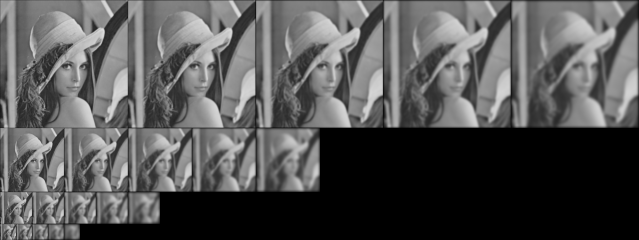
\includegraphics{../images/LenaGaussianPyramid.png}\\
          (a)
        \end{center}
      \end{minipage}    \\
      \begin{minipage}{1\hsize}
        \begin{center}
          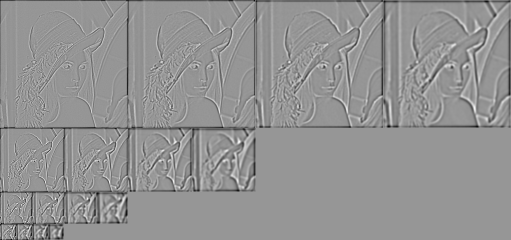
\includegraphics{../images/LenaDoGPyramid.png}\\
          (b)
        \end{center}
      \end{minipage}    
    \end{tabular}
    \caption{
      The result of the first step of SIFT computation. 
      Pyramids generated with 4 levels (or octaves) and the number of intervals, $s$, is 2. 
      (a) Gaussian Pyramid. The number of Gaussian functions in each level is $s+3=5$. 
      (b) DoG Pyramid. The number of DoG function in each level is $s+2=4$. 
    }
    \label{Fi:PYR}
  \end{center}
\end{figure*} 

\begin{figure*}[p]
  \begin{center}
    \begin{tabular}{@{} ccc @{}}

      \begin{minipage}{0.33\hsize}
        \begin{center}
          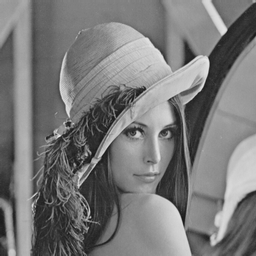
\includegraphics[width=5cm]{../images/Lena.png}\\
          (a)
        \end{center}
      \end{minipage}    &
      \begin{minipage}{0.33\hsize}
        \begin{center}
          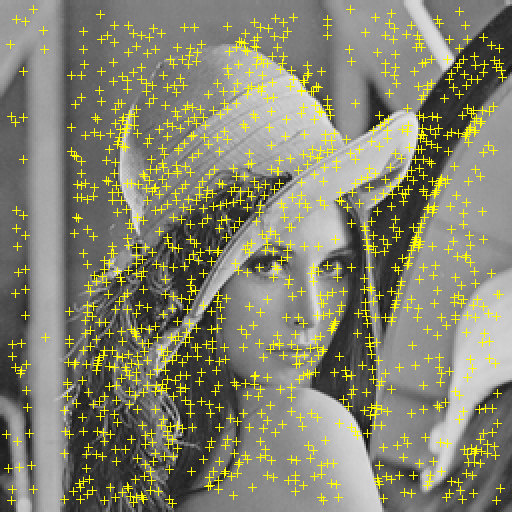
\includegraphics[width=5cm]{../images/LenaKeypointExtrema.png}\\
          (b)
        \end{center}
      \end{minipage}    &
      \begin{minipage}{0.33\hsize}
        \begin{center}
          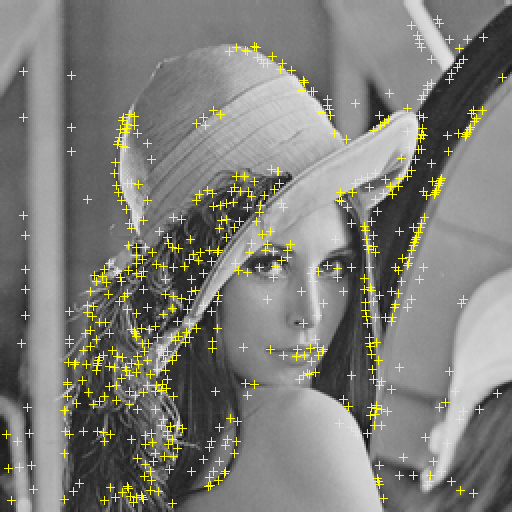
\includegraphics[width=5cm]{../images/LenaKeypointRemoveLowContrast.png}\\
          (c)
        \end{center}
      \end{minipage}    \\
      \begin{minipage}{0.33\hsize}
        \begin{center}
          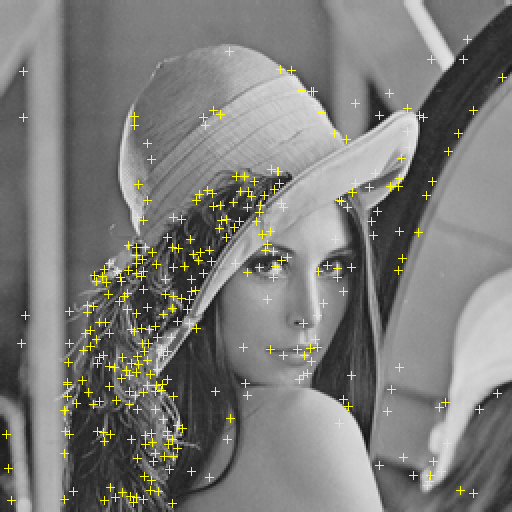
\includegraphics[width=5cm]{../images/LenaKeypointRemoveEdge.png}\\
          (d)
        \end{center}
      \end{minipage}    &
      \begin{minipage}{0.33\hsize}
        \begin{center}
          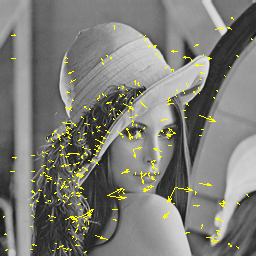
\includegraphics[width=5cm]{../images/LenaOrientation.png}\\  
          (e)
        \end{center}
      \end{minipage}    &
    \end{tabular}
    \caption{
      The result of the second (b-d) and the third (e) step of the SIFT computation.
      (a) Input Image
      (b) Detected DoG extrema points (1294 points) 
      (c) After removing low contrast extrema with threshold 0.03 (605 points)
      (d) After removing edge points with curvature ratio $ r = 10.0 $ (328 points)
      (e) Orientation Assignment
    }
    \label{Fi:KEY}
  \end{center}
\end{figure*} 

%%%%%%%% Interest point detector

\begin{figure*}[p]
  \begin{center}
    \begin{tabular}{@{} cc @{}}

      \begin{minipage}{0.5\hsize}
        \begin{center}
          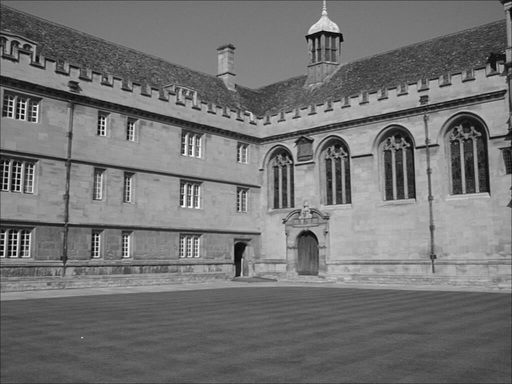
\includegraphics[width=7cm]{../images/wadham001.png}\\
          (a)
        \end{center}
      \end{minipage}    &
      \begin{minipage}{0.5\hsize}
        \begin{center}
          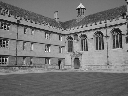
\includegraphics[width=2cm]{../images/wadham001S.png}\\
          (b)
        \end{center}
      \end{minipage}    \\
      \begin{minipage}{0.5\hsize}
        \begin{center}
          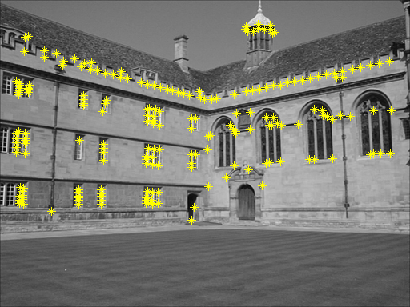
\includegraphics[width=7cm]{../images/Harriswadham001.png}\\
          (c)
        \end{center}
      \end{minipage}    &
      \begin{minipage}{0.5\hsize}
        \begin{center}
          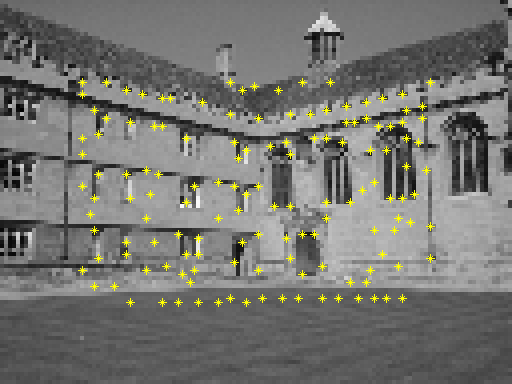
\includegraphics[width=7cm]{../images/Harriswadham001S.png}\\
          (d)
        \end{center}
      \end{minipage}    \\
      \begin{minipage}{0.5\hsize}
        \begin{center}
          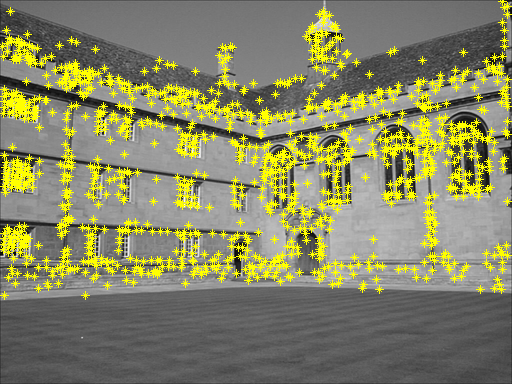
\includegraphics[width=7cm]{../images/SIFTwadham001.png}\\
          (e)
        \end{center}
      \end{minipage}    &
      \begin{minipage}{0.5\hsize}
        \begin{center}
          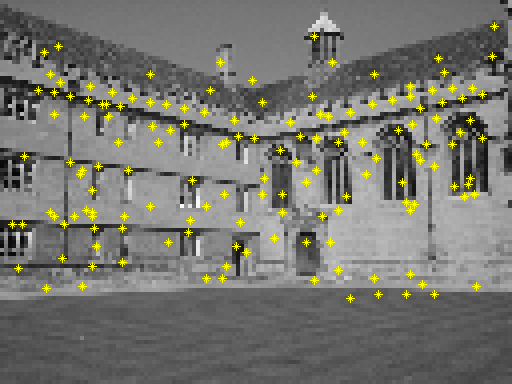
\includegraphics[width=7cm]{../images/SIFTwadham001S.png}\\
          (f)
        \end{center}    
      \end{minipage}    \\
    \end{tabular}
    \caption{
      Comparison between Harris corner detection and SIFT as an interest point detector. 
      (a) Input image. 
      (b) Scale downed input image (25\%). 
      (c) The Result of the Harris corner detection applied to (a). 
      (d) The Result applied to scale downed image, and resized. 
      The average least distance error between results of (c) and (d) is 20.7919. 
      (e) The Result of the SIFT after keypoint detection step applied to (a). 
      (f) The Result applied to scale downed image, and resized.  
      The average least distance error between results of (e) and (f) is 4.4997. 
    }
    \label{Fi:EXPINT}
  \end{center}
\end{figure*} 

%%%%%%%% Image matching

\begin{figure*}[p]
  \begin{center}
    \begin{tabular}{@{} c @{}}

      \begin{minipage}{1.0\hsize}
        \begin{center}
          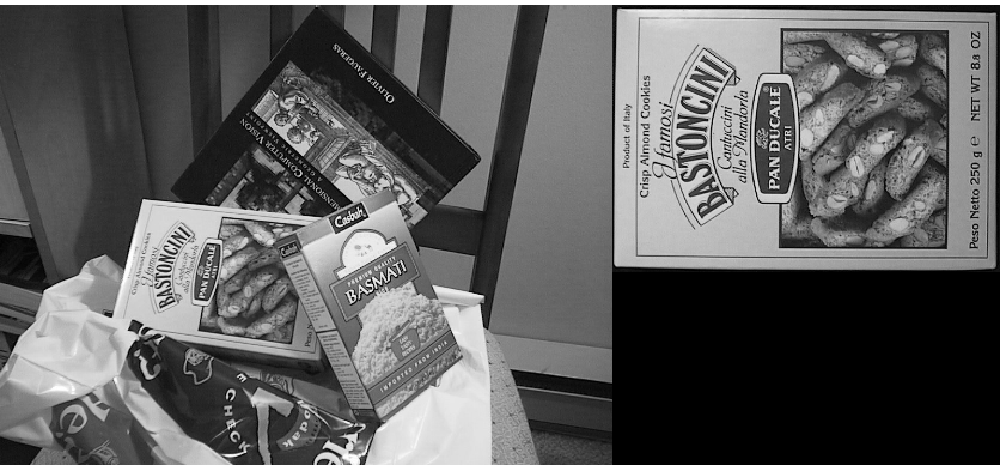
\includegraphics[width=13cm]{../images/BookScene.png}\\
          (a)
        \end{center}
      \end{minipage}    \\
      \begin{minipage}{1.0\hsize}
        \begin{center}
          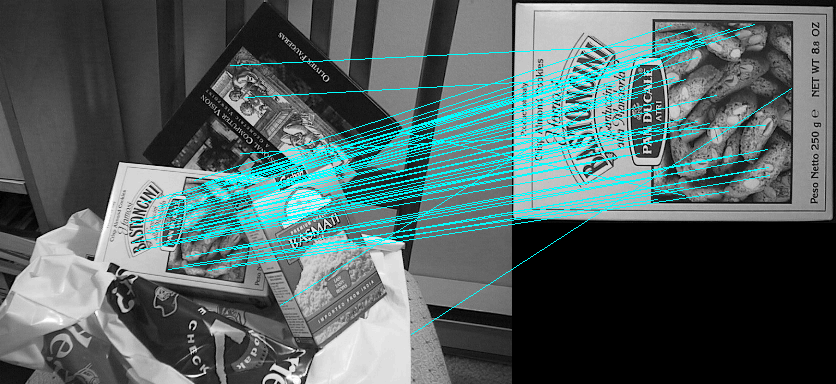
\includegraphics[width=13cm]{../images/BookSceneMatch.png}\\
          (b)
        \end{center}
      \end{minipage}    \\
      \begin{minipage}{1.0\hsize}
        \begin{center}
          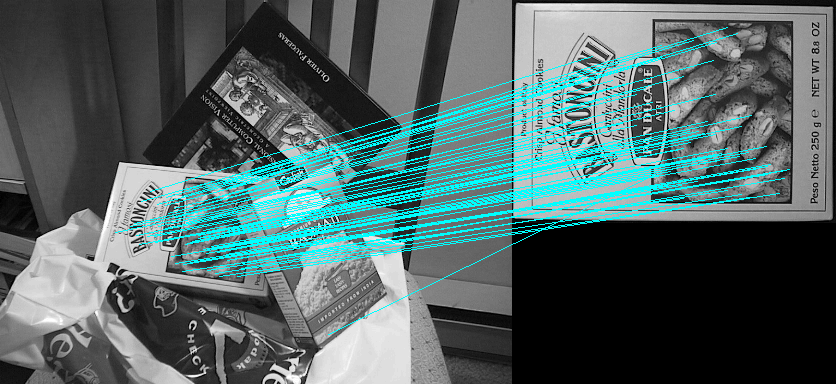
\includegraphics[width=13cm]{../images/BookSceneMatchLowe.png}\\
          (c)
        \end{center}
      \end{minipage}    \\
    \end{tabular}
    \caption{
      Image Matching based on SIFT: Comparison with a ground truth
      (a) Input Images
      (b) Result of image matching obtained by our implementation
      (c) Result of image matching obtained by Lowe's software \cite{dLowe05}
    }
    \label{Fi:MATCH}
  \end{center}
\end{figure*} 

\begin{figure*}[p]
  \begin{center}
    \begin{tabular}{@{} c @{}}

      \begin{minipage}{1.0\hsize}
        \begin{center}
          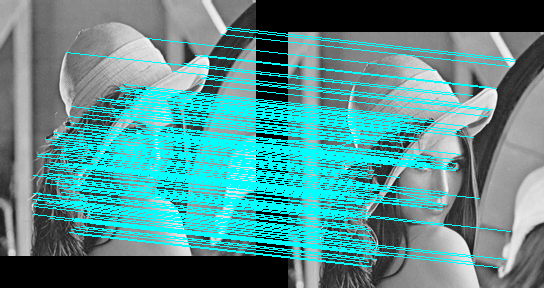
\includegraphics{../images/HarrisTranslationInvariantTest.png}\\
          (a)
        \end{center}
      \end{minipage}    \\
      \begin{minipage}{1.0\hsize}
        \begin{center}
          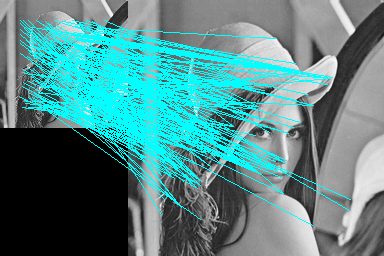
\includegraphics{../images/HarrisScaleInvariantTest05.png}\\
          (b)
        \end{center}
      \end{minipage}    \\
      \begin{minipage}{1.0\hsize}
        \begin{center}
          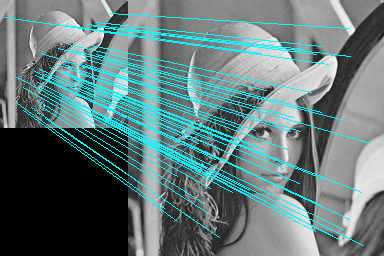
\includegraphics{../images/SIFTScaleInvariantTest05.png}\\
          (c)
        \end{center}
      \end{minipage}    \\
    \end{tabular}
    \caption{
      Invariant Property Test
      (a) Translation invariant test for our Harris based method
      (b) Our Harris based method is feasible (non-invariant) to scale change
      (c) SIFT is invariant to scale (correct corresponding will not create crossing lines)
    }
    \label{Fi:INVARIANT}
  \end{center}
\end{figure*} 

%%%%%%%%%% Tracking

\begin{figure*}[p]
  \begin{center}
    \begin{tabular}{@{} ccc @{}}

      \begin{minipage}{0.33\hsize}
        \begin{center}
          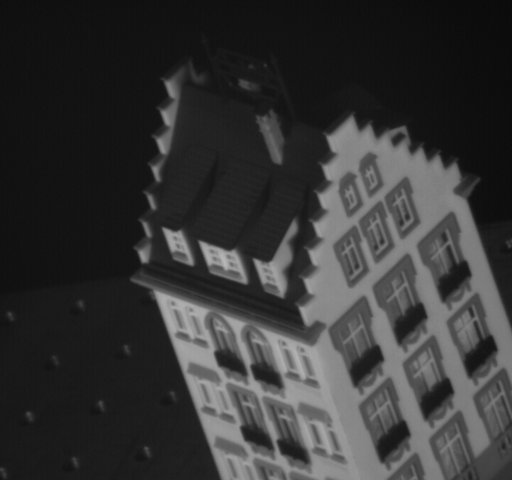
\includegraphics[width=5cm]{../../images/hotel/hotel1.png}\\
          (a)
        \end{center}
      \end{minipage}    &
      \begin{minipage}{0.33\hsize}
        \begin{center}
          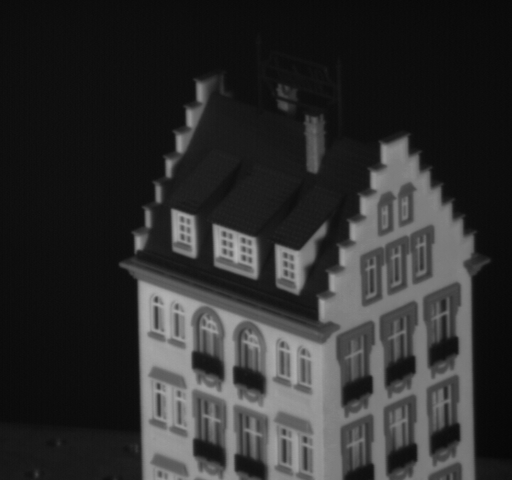
\includegraphics[width=5cm]{../../images/hotel/hotel50.png}\\
          (b)
        \end{center}
      \end{minipage}    
      \begin{minipage}{0.33\hsize}
        \begin{center}
          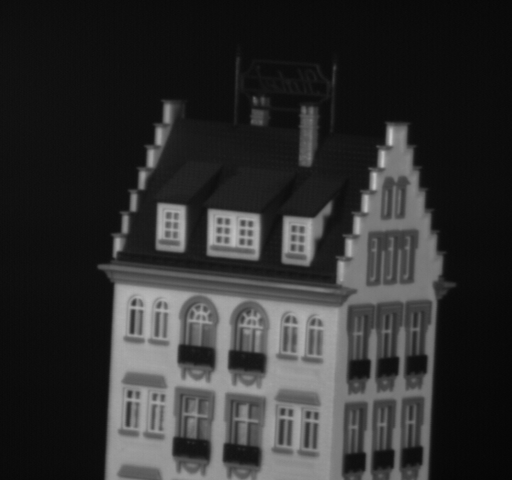
\includegraphics[width=5cm]{../../images/hotel/hotel100.png}\\
          (c)
        \end{center}
      \end{minipage}    
    \end{tabular}
    \caption{baseline Hotel image sequence
      (a) The 1st frame
      (b) The 50th frame
      (c) The 100th frame
    } 
    \label{fig:BaseLine}
  \end{center}
\end{figure*} 

\begin{figure*}[p]
  \begin{center}
    \begin{tabular}{@{} cc @{}}

      \begin{minipage}{0.5\hsize}
        \begin{center}
          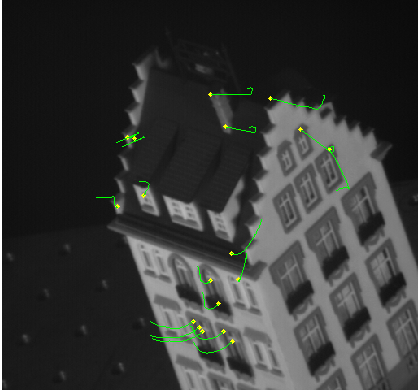
\includegraphics[width=8cm]{../../images/hotel/hoteltracked100.png}\\
          (a)
        \end{center}
      \end{minipage}    &
      \begin{minipage}{0.5\hsize}
        \begin{center}
          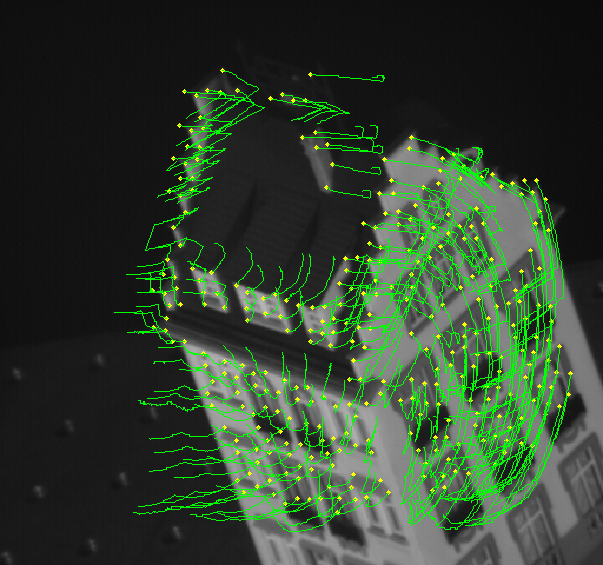
\includegraphics[width=8cm]{../../images/hotel/klttrack.png}\\
          (b)
        \end{center}
      \end{minipage}    
    \end{tabular}
    \caption{
      Interest point tracking. The first frame picture is shown, and starting points are shown by star (yellow) points, tracking results are shown by lines (green). 
      (a) Result of the point tracking based on SIFT (18 points remained). 
      (b) Result of KLT Point Tracker (248 points remained). 
      About 500 interest points were detected in each frame on both SIFT and KLT. 
    } 
    \label{Fi:hoteltracks}
  \end{center}
\end{figure*}

\begin{figure*}[p]
  \begin{center}
    \begin{tabular}{@{} ccc @{}}

      \begin{minipage}{0.33\hsize}
        \begin{center}
          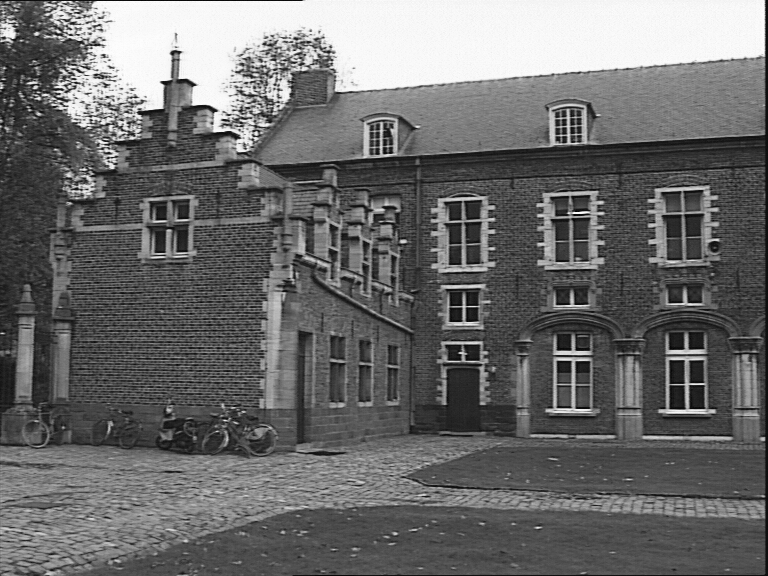
\includegraphics[width=5cm]{../../images/castle/castle001.png}\\
          (a)
        \end{center}
      \end{minipage}    &
      \begin{minipage}{0.33\hsize}
        \begin{center}
          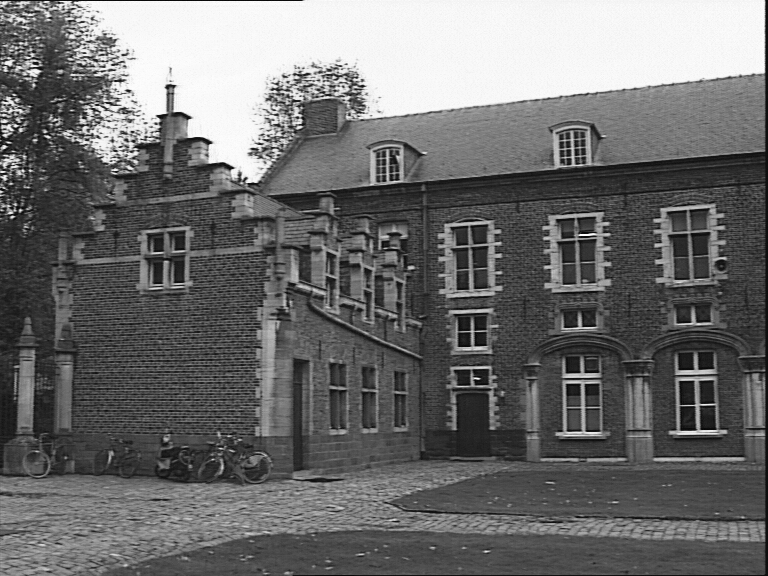
\includegraphics[width=5cm]{../../images/castle/castle002.png}\\
          (b)
        \end{center}
      \end{minipage}    
      \begin{minipage}{0.33\hsize}
        \begin{center}
          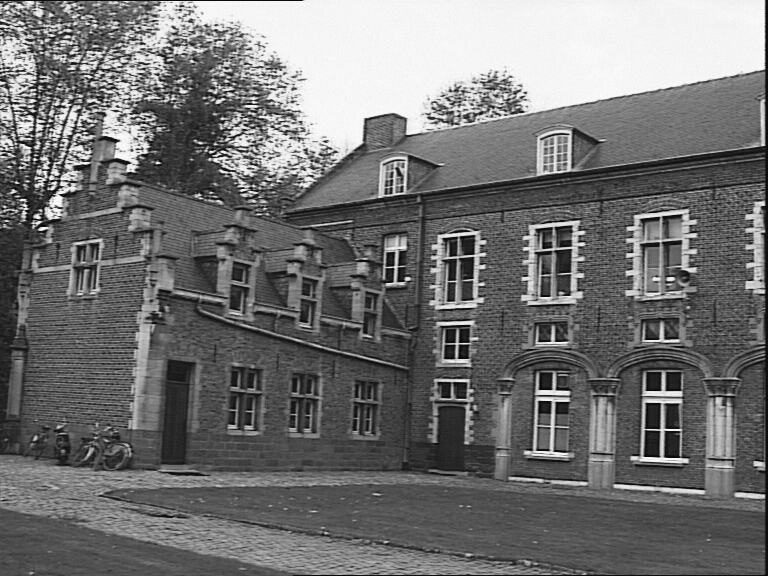
\includegraphics[width=5cm]{../../images/castle/castle013.png}\\
          (c)
        \end{center}
      \end{minipage}    
    \end{tabular}
    \caption{baseline Castle image sequence, totally 13 frames. 
      (a) The 1st frame
      (b) The 2nd frame
      (c) The 13th frame
    } 
    \label{fig:CastleBaseLine}
  \end{center}
\end{figure*} 

\begin{figure*}[p]
  \begin{center}
    \begin{tabular}{@{} cc @{}}

      \begin{minipage}{0.5\hsize}
        \begin{center}
          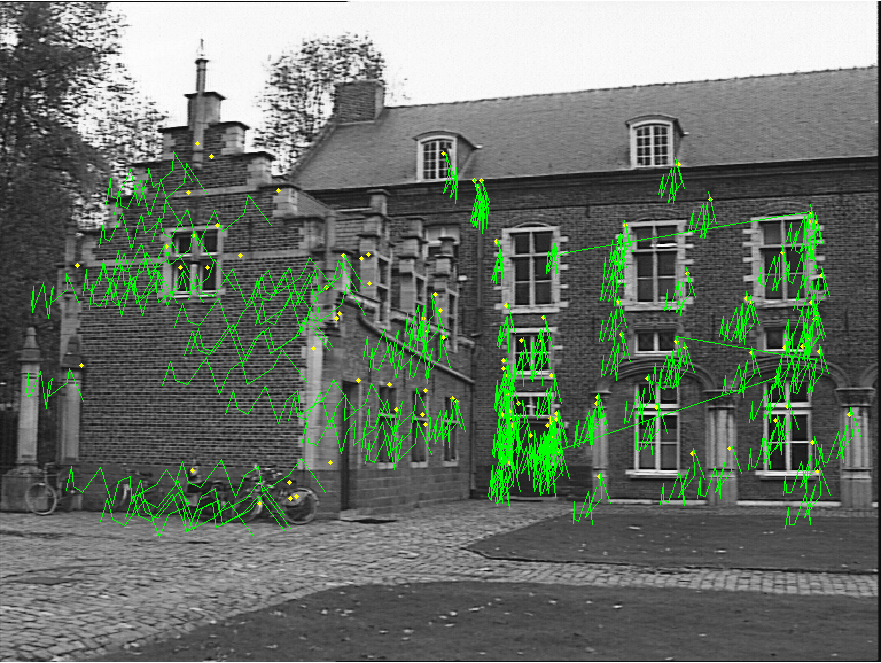
\includegraphics[width=8cm]{../../images/castle/SIFTcastle.png}\\
          (a)
        \end{center}
      \end{minipage}    &
      \begin{minipage}{0.5\hsize}
        \begin{center}
          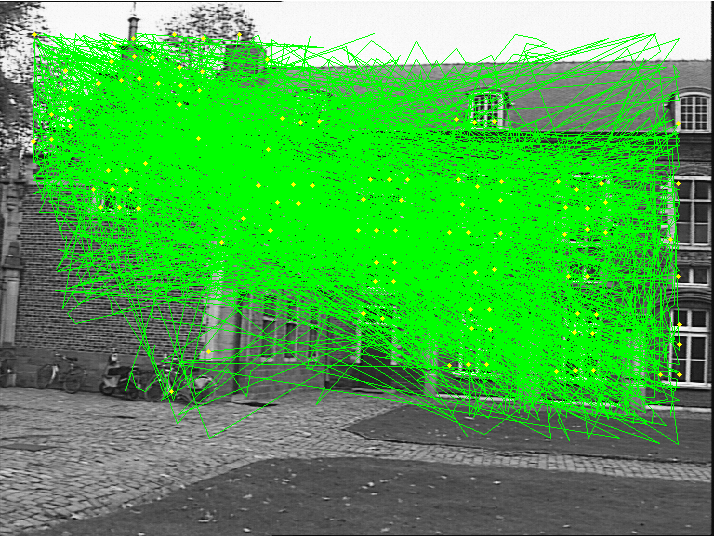
\includegraphics[width=8cm]{../../images/castle/KLTcastle.png}\\
          (b)
        \end{center}
      \end{minipage}    
    \end{tabular}
    \caption{
      Interest point tracking. The first frame picture is shown, and starting points are shown by star (yellow) points, tracking results are shown by lines (green). 
      (a) Result of the point tracking based on SIFT (83 points remained). 
      (b) Result of KLT Point Tracker (131 points remained). 
      About 5000 interest points were detected in each frame on both SIFT and KLT. 
    } 
    \label{Fi:castletracks}
  \end{center}
\end{figure*}

%%%%%%%% Panorama

\begin{figure*}[p]
  \begin{center}
    \begin{tabular}{@{} ccc @{}}

      \begin{minipage}{0.33\hsize}
        \begin{center}
          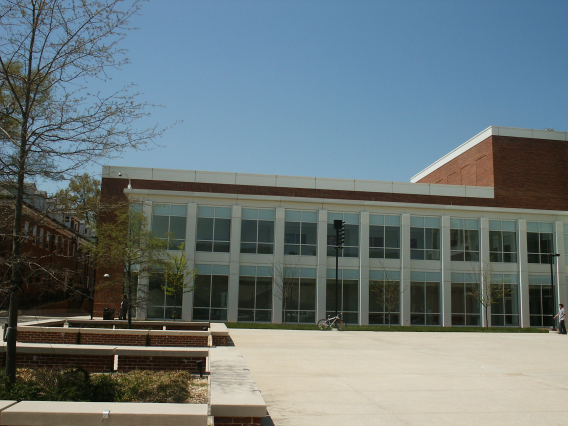
\includegraphics[width=5cm]{../../images/KIM/KIM3.png}\\
          ~
        \end{center}
      \end{minipage}    &
      \begin{minipage}{0.33\hsize}
        \begin{center}
          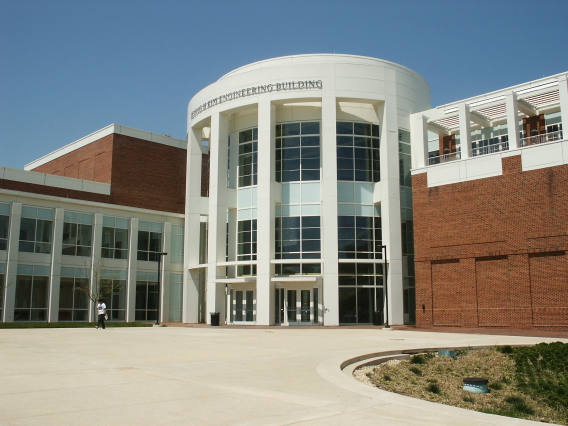
\includegraphics[width=5cm]{../../images/KIM/KIM2.png}\\
          (a)
        \end{center}
      \end{minipage}    &
      \begin{minipage}{0.33\hsize}
        \begin{center}
          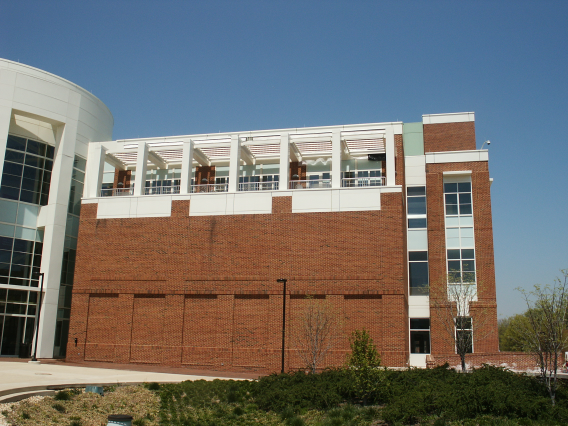
\includegraphics[width=5cm]{../../images/KIM/KIM1.png}\\
          ~
        \end{center}
      \end{minipage}    \\
      \multicolumn{3}{c}{
      \begin{minipage}{1.0\hsize}
        \begin{center}
          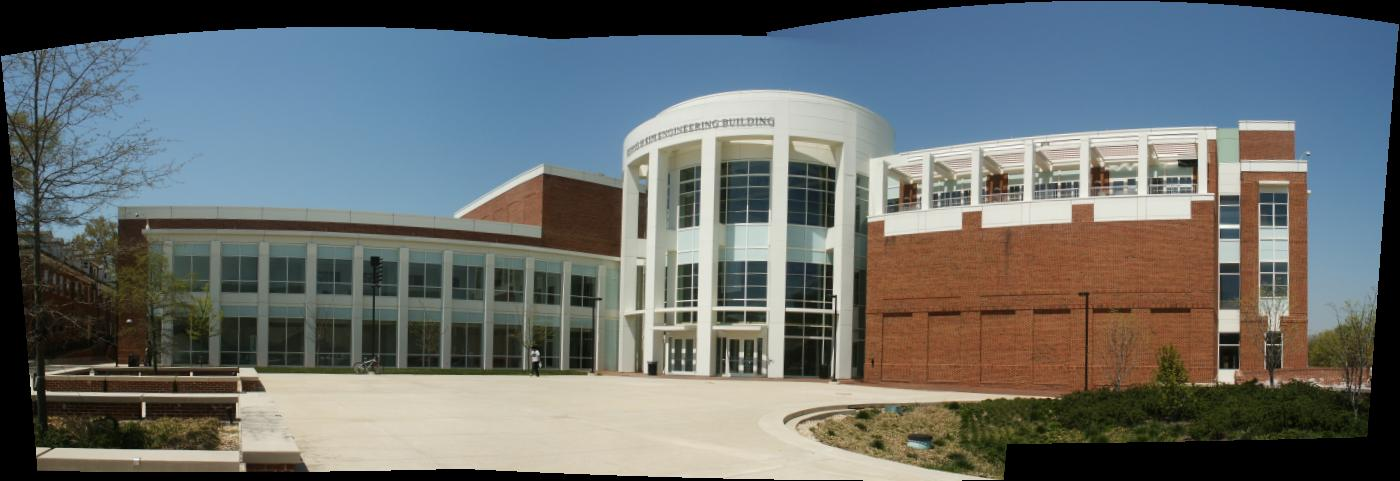
\includegraphics[width=15cm]{../../images/KIM/pano.jpg}\\
          (b)
        \end{center}
      \end{minipage}    
      }\\
    \end{tabular}
    \caption{
      Panoramic Image Stitching
      (a) Input Images - KIM building at the University of Maryland
      (b) Result
    } 
    \label{Fi:Panorama}
  \end{center}
\end{figure*} 

\end{document}
